\section{Graph Nomenclature}%
\label{sec:graph_nomenclature}

\begin{frame}
	\frametitle{A Graph}

	\begin{columns}
		\column{0.405\textwidth}
		\begin{tikzpicture}[scale=0.8, transform shape]
	\begin{scope}[every node/.style={circle,thick,draw,onslide=<2>{draw=red}}]
    \node (A) at (0,0) {A};
    \node (B) at (0,3) {B};
    \node (C) at (2.5,4) {C};
    \node (D) at (2.5,1) {D};
    \node (E) at (2.5,-3) {E};
    \node (F) at (5,3) {F} ;
\end{scope}

\begin{scope}[>={Stealth},
              every node/.style={fill=white,circle},
							every edge/.style={very thick, draw=black,onslide=<3>{draw=red}}]
    \path (A) edge (B);
    \path (B) edge (C);
    \path (A) edge (D);
    \path (D) edge (C);
    \path (A) edge (E);
    \path (D) edge (E);
    \path (D) edge (F);
    \path (C) edge (F);
    \path (E) edge (F); 
    \path (B) edge[bend right=60] (E); 
\end{scope}
\end{tikzpicture}

		\column{0.605\textwidth}
		\begin{itemize}
			\item A graph is just a bunch of circles and lines.
				\pause
			\item These circles are called \alert{vertices} (or \alert{nodes}).
				\pause
			\item These lines are called \alert{edges} (or \alert{connections}).
				\pause
			\item In this form the graph is called \textit{undirected} and \textit{unweighted}.
		\end{itemize}
	\end{columns}
\end{frame}

\begin{frame}
	\frametitle{Directed Graphs}
	
	\begin{columns}
		\column{0.405\textwidth}
		\alt<2>{
			\begin{tikzpicture}[scale=0.8, transform shape]
\begin{scope}[every node/.style={circle,thick,draw}]
    \node (A) at (0,0) {A};
    \node (B) at (0,3) {B};
    \node (C) at (2.5,4) {C};
    \node (D) at (2.5,1) {D};
    \node (E) at (2.5,-3) {E};
    \node (F) at (5,3) {F} ;
\end{scope}

\begin{scope}[>={Stealth[black]},
              every node/.style={fill=white,circle},
              every edge/.style={draw=black,very thick}]
    \path [->] (A) edge node {$5$} (B);
    \path [->] (B) edge node {$3$} (C);
    \path [->] (A) edge node {$4$} (D);
    \path [->] (D) edge node {$3$} (C);
    \path [->] (A) edge node {$3$} (E);
    \path [->] (D) edge node {$3$} (E);
    \path [->] (D) edge node {$3$} (F);
    \path [->] (C) edge node {$5$} (F);
    \path [->] (E) edge node {$8$} (F); 
    \path [->] (B) edge[bend right=60] node {$1$} (E); 
\end{scope}
\end{tikzpicture}

			}{
			\begin{tikzpicture}[scale=0.8, transform shape]
	\begin{scope}[every node/.style={circle,thick,draw}]
    \node (A) at (0,0) {A};
    \node (B) at (0,3) {B};
    \node (C) at (2.5,4) {C};
    \node (D) at (2.5,1) {D};
    \node (E) at (2.5,-3) {E};
    \node (F) at (5,3) {F} ;
\end{scope}

\begin{scope}[>={Stealth},
              every node/.style={fill=white,circle},
							every edge/.style={draw=black,very thick}]
							\path[->] (A) edge (B);
							\path[->] (B) edge (C);
							\path[->] (A) edge (D);
							\path[->] (D) edge (C);
							\path[->] (A) edge (E);
							\path[->] (D) edge (E);
							\path[->] (D) edge (F);
							\path[->] (C) edge (F);
							\path[->] (E) edge (F); 
							\path[->] (B) edge[bend right=60] (E); 
\end{scope}
\end{tikzpicture}

		}
		\column{0.605\textwidth}
		\begin{itemize}
			\item Edges can also have a direction.
			\item In which case we call it a \textit{directed} graph.
				\pause
			\item Furthermore they can have weights.
			\item In which case we call it a \textit{weighted} graph.
		\end{itemize}
	\end{columns}
\end{frame}

\begin{frame}
	\frametitle{Let's formalise!}

		\begin{block}{A formal definition of a graph}
			\begin{itemize}
				\item A graph $G=(V,E)$, where:
					\begin{itemize}
						\item $V$ is a set of vertices,
						\item $E$ is a set of edges, where every edge has two \textit{endpoints}.
					\end{itemize}
					\pause
				\item If the graph is \textit{weighted} then there is a function $w: E \to \mathbb{R}$ which maps every edge to
					a weight.
					\pause
					\begin{itemize}
						\item In most cases we will restrict ourselves to functions $w: E \to \mathbb{N}$, i.e. non-negative integer weights.
					\end{itemize}
					\pause
				\item Depending on direction:
					\begin{itemize}
					\pause
						\item If the graph is \textit{directed} then every edge $e = (u,v)$ with $u,v \in V$. In this case we call
							$u$ the \textit{origin} and $v$ the \textit{destination}
					\pause
				\item If the graph is \textit{undirected} then every edge $e = \{u,v\}$ with $u,v \in V$.\footnote{Unfortunately
						in many textbooks/papers/slides people also use $e=(u,v)$ for undirected edges, but just remark they are
					undirected.}
					\end{itemize}
			\end{itemize}
		\end{block}	
\end{frame}

\begin{frame}
	\frametitle{Let's draw}

	\begin{problemblock}{Just like Toothless}
		Draw the following graph:
		\begin{itemize}
			\item $V = \{A,B,C,D,E,F\}$\\
			\item	$E = \{
			\{A, B\},
			\{A, D\},
			\{D, C\},
			\{B, F\},
			\{B, E\},$\\$
			\{E, D\},
			\{E, F\},
			\{C, F\},
			(A,C),
			(C,A),
			(D,B),
			(B,C)
		\}$\\
	\item $w(\{E,D\}) = 8$, $w((A,C)) = 2$, $w(\{C,F\}) = 5$, $w(\{E,B\}) = 2$, $w((C,A)) = 8$.
		For all other edges $e$, $w(e) = 1$.
		\end{itemize}
	\end{problemblock}
\end{frame}

\begin{frame}
	\frametitle{Properties of vertices}
		
	\begin{columns}
		\column{0.405\textwidth}
			\begin{tikzpicture}[scale=0.8, transform shape]
	\begin{scope}[every node/.style={circle,thick,draw}]
		\node[onslide=<2-3>{draw=red}] (A) at (0,0) {A};
    \node (B) at (0,3) {B};
    \node[onslide=<4-5>{draw=red}] (C) at (2.5,4) {C};
		\node[onslide=<2>{draw=red}] (D) at (2.5,1) {D};
    \node (E) at (2.5,-3) {E};
    \node (F) at (5,3) {F} ;
\end{scope}

\begin{scope}[>={Stealth},
              every node/.style={fill=white,circle},
							every edge/.style={draw=black,very thick}]
							\path[onslide=<4->{->}] (A) edge[onslide=<3>{draw=red}] (B);
							\path[onslide=<4->{->}] (B) edge[onslide=<4>{draw=red}] (C);
							\path[onslide=<4->{->}] (A) edge[onslide=<3>{draw=red}] (D);
							\path[onslide=<4->{->}] (D) edge[onslide=<4>{draw=red}] (C);
							\path[onslide=<4->{->}] (A) edge[onslide=<3>{draw=red}] (E);
							\path[onslide=<4->{->}] (D) edge (E);
							\path[onslide=<4->{->}] (D) edge (F);
							\path[onslide=<4->{->}] (C) edge[onslide=<5>{draw=red}] (F);
							\path[onslide=<4->{->}] (E) edge (F); 
							\path[onslide=<4->{->}] (B) edge[bend right=60] (E); 
\end{scope}
\end{tikzpicture}

		\column{0.605\textwidth}
		Vertices also have some properties:
		\pause
		\begin{itemize}
			\item Two vertices are \alert{adjacent} if there is an edge between them.
			\item We also call these \alert{neighbouring} vertices.
				\pause
			\item Every vertex has a set of \alert{incident} edges, namely those connected to it.
				\pause
			\item If the graph is directed, we can split this into:
				\begin{itemize}
					\item \alert{incoming} edges.
						\pause
					\item \alert{outgoing} edges.
				\end{itemize}
		\end{itemize}
	\end{columns}
\end{frame}

\begin{frame}
	\frametitle{More formalisation}
	\begin{block}{Properties of vertices}
		\begin{itemize}
			\item Two vertices $u,v \in V$ are adjacent, or neighbours, iff $\exists e \in E$ s.t. $e=(u,v)$.
				\pause
			\item The set of neighbours of $u$ is all of the nodes $v \in V$ that are neighbours of $u$.
				\pause
			\item An edge $e$ is incident to a vertex $v$ if $e=(u,v)$ or $e = (v,u)$ for some $u \in V$.
				\pause
			\item The \alert{degree} of a vertex $v$ is the number of incident edges to $v$, so $\mathit{deg}: V \to \mathbb{N}$.
				\pause
			\item For a directed graph, we define $\mathit{indeg}: V \to \mathbb{N}$ and $\mathit{outdeg}: V \to \mathbb{N}$,
				such that:
				\pause
				\begin{itemize}
					\item $\mathit{indeg}(v) = | \{u \mid (u,v) \in E\}|$
					\item $\mathit{outdeg}(v) = | \{u \mid (v,u) \in E\}|$
						\pause
					\item This means that: $\mathit{indeg}(v) + \mathit{outdeg}(v) = \mathit{deg}(v)$.
				\end{itemize}
		\end{itemize}
	\end{block}	
\end{frame}

\begin{frame}
	\frametitle{Lets check again}
	\begin{columns}
		\column{0.405\textwidth}
			\begin{tikzpicture}[scale=0.8, transform shape]
	\begin{scope}[every node/.style={circle,thick,draw}]
		\node[] (A) at (0,0) {A};
    \node (B) at (0,3) {B};
    \node[] (C) at (2.5,4) {C};
		\node[] (D) at (2.5,1) {D};
    \node (E) at (2.5,-3) {E};
    \node (F) at (5,3) {F} ;
\end{scope}

\begin{scope}[>={Stealth[black]},
              every node/.style={fill=white,circle},
							every edge/.style={draw=black,very thick}]
							\path[->] (A) edge (B);
							\path[->] (B) edge (C);
							\path[->] (A) edge (D);
							\path[->] (D) edge (C);
							\path[->] (A) edge (E);
							\path[->] (D) edge (E);
							\path[->] (D) edge (F);
							\path[->] (C) edge (F);
							\path[->] (E) edge (F); 
							\path[->] (B) edge[bend right=60] (E); 
\end{scope}
\end{tikzpicture}

		\column{0.605\textwidth}
	\begin{questionblock}{What dos the following result in?}
	\pause
		$\mathit{outdeg}(D) + \mathit{indeg}(C) + \sum\limits_{v\in \{v \in V \mid (B,v) \in E\}} \mathit{deg}(v) = $
		\begin{enumerate}[A.]
			\item 4
			\item 8
			\item 12
			\item 16
			\item I don't know.
		\end{enumerate}
	\end{questionblock}
	\pause
	\begin{answerblock}{If I did my math right...}
		3 leaving $D$, 2 entering $C$ and the degrees of C and E (3 and 4) makes 12.
	\end{answerblock}
	\end{columns}
\end{frame}

\begin{frame}
	\frametitle{There are extensions/special cases}
	\begin{columns}
		\column{0.405\textwidth}
			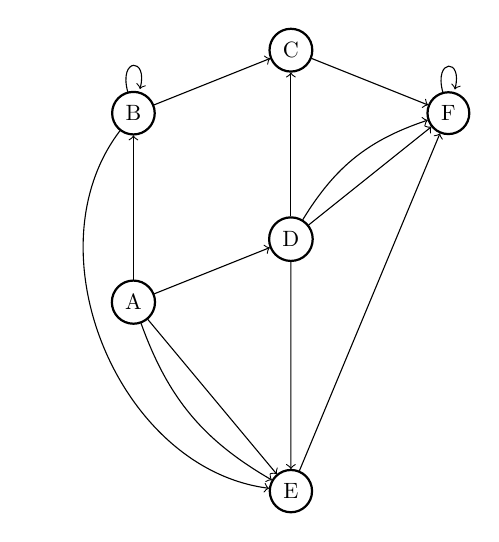
\begin{tikzpicture}[scale=0.8, transform shape]
	\begin{scope}[every node/.style={circle,thick,draw}]
		\node[] (A) at (0,0) {A};
    \node (B) at (0,3) {B};
    \node[] (C) at (2.5,4) {C};
		\node[] (D) at (2.5,1) {D};
    \node (E) at (2.5,-3) {E};
    \node (F) at (5,3) {F} ;
\end{scope}

\begin{scope}[
              every node/.style={fill=white,circle},
							every edge/.style={draw=black}]
							\path[->] (A) edge (B);
							\path[->] (B) edge (C);
							\path[->] (A) edge (D);
							\path[->] (D) edge (C);
							\path[->] (A) edge (E);
							\onslide<2>{\path[->] (A) edge[bend right=20] (E);}
							\path[->] (D) edge (E);
							\path[->] (D) edge (F);
							\onslide<2>{\path[->] (D) edge[bend left=20] (F);}
							\path[->] (C) edge (F);
							\path[->] (E) edge (F); 
							\path[->] (B) edge[bend right=60] (E); 
							\onslide<3>{\path[->] (B) edge[ loop above] (B);}
							\onslide<3>{\path[->] (F) edge[ loop above] (F);}
\end{scope}
\end{tikzpicture}

		\column{0.605\textwidth}
		\begin{itemize}
			\item A graph can also have a \textit{collection} of edges, rather than a set. We call this a \textit{multigraph}.
				\pause
			\item This allows multiple edges between the same pair of nodes.
				\pause
			\item Some versions also allow \textit{self-loops}.
				\pause
			\item But in our course we mostly consider \alert{simple} graphs, where $E$ is a set and there are no self-loops.
		\end{itemize}
	\end{columns}
\end{frame}

\begin{frame}
	\frametitle{Putting some edges together}
	\begin{columns}
		\column{0.405\textwidth}
			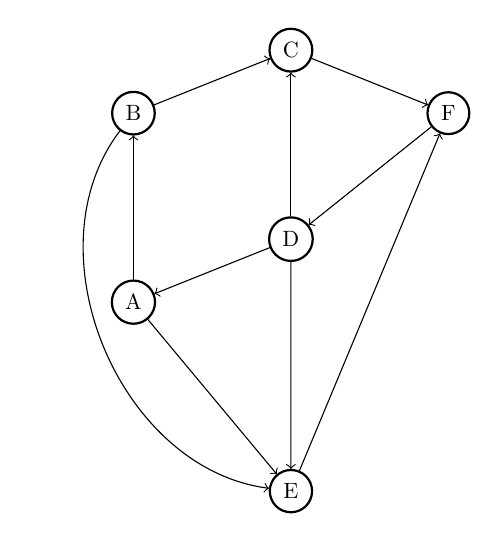
\begin{tikzpicture}[scale=0.8, transform shape]
	\begin{scope}[every node/.style={circle,thick,draw}]
		\node[] (A) at (0,0) {A};
    \node (B) at (0,3) {B};
    \node[] (C) at (2.5,4) {C};
		\node[] (D) at (2.5,1) {D};
    \node (E) at (2.5,-3) {E};
    \node (F) at (5,3) {F} ;
\end{scope}

\begin{scope}[
              every node/.style={fill=white,circle},
							every edge/.style={draw=black}]
							\path[->] (A) edge[] (B);
							\path[->] (B) edge[] (C);
							\path[->] (D) edge[] (A);
							\path[->] (D) edge (C);
							\path[->] (A) edge[] (E);
							\path[->] (D) edge (E);
							\path[->] (F) edge[] (D);
							\path[->] (C) edge[] (F);
							\path[->] (E) edge (F); 
							\path[->] (B) edge[bend right=60] (E); 
\end{scope}
\end{tikzpicture}

		\column{0.605\textwidth}
		\begin{itemize}
			\item A \textit{path} is a sequence of edges, connected to each other.
				\pause
			\item Paths can even contain the same nodes twice.
			\item The path in \alert{red} starts at $A$ and ends at $E$.
				\pause
			\item \textit{Cycles} are paths that start and end at the same vertex.
				\pause
			\item Simple paths and simple cycles allow every vertex at most once (with the exception for a cycle, where the
				starting vertex is equal to the ending vertex).
		\end{itemize}
	\end{columns}
\end{frame}

\begin{frame}
	\frametitle{Almost done!}
	\begin{block}{Paths}
		\begin{itemize}
			\item A path $\pi$ is commonly denoted as a sequence of vertices (in simple graphs), or a sequence of edges (in
				multi-graphs).
				\pause
			\item If denoted as a sequence of vertices, then $\pi$ is a path iff for every consecutive vertices $u,v$ in the
				sequence, $\{u,v\} \in E$.
				\pause
			\item If denoted as a sequence of edges, then $\pi$ is a path iff for every consecutive edges $e,f$ in the
				sequence, $e=\{u,v\}, f=\{v,w\}$ for some $u,v,w \in V$.
				\pause
			\item A cycle is a path $\pi = \{v_1, \dots, v_1\}$ (when denoted as a sequence of vertices).
				\pause
			\item For a directed graph, we can also speak of \textit{directed paths} and \textit{directed cycles}.
		\end{itemize}
	\end{block}	
\end{frame}

\begin{frame}
	\frametitle{The longest path}
	\begin{columns}
		\column{0.405\textwidth}
			\begin{tikzpicture}[scale=0.8, transform shape]
	\begin{scope}[every node/.style={circle,thick,draw}]
		\node[] (A) at (0,0) {A};
    \node (B) at (0,3) {B};
    \node[] (C) at (2.5,4) {C};
		\node[] (D) at (2.5,1) {D};
    \node (E) at (2.5,-3) {E};
    \node (F) at (5,3) {F} ;
\end{scope}

\begin{scope}[>={Stealth},
              every node/.style={fill=white,circle},
							every edge/.style={draw=black,very thick}]
							\path[->] (A) edge[onslide=<3>{draw=red}] (B);
							\path[->] (B) edge[onslide=<3>{draw=red}] (C);
							\path[->] (D) edge (A);
							\path[->] (D) edge (C);
							\path[->] (A) edge (E);
							\path[->] (D) edge[onslide=<3>{draw=red}] (E);
							\path[->] (F) edge[onslide=<3>{draw=red}] (D);
							\path[->] (C) edge[onslide=<3>{draw=red}] (F);
							\path[->] (E) edge (F); 
							\path[->] (B) edge[bend right=60] (E); 
\end{scope}
\end{tikzpicture}

		\column{0.605\textwidth}
		\begin{questionblock}{Longest path?}
		\pause
			How many vertices are part of the longest simple path in this graph?
			\begin{enumerate}[A.]
				\item 4
				\item 5 
				\item 6
				\item 7
				\item I don't know.
			\end{enumerate}
		\end{questionblock}
		\pause
		\vspace{-10pt}
		\begin{answerblock}{All of them}
			In this case 6. \\
			Fun fact: this is actually a \alert{very very hard problem} that Computer Scientists cannot solve efficiently. More
			information on this when we discuss P vs NP.
		\end{answerblock}
	\end{columns}
\end{frame}

\begin{frame}
	\frametitle{Finally we have reached the end}

		\begin{block}{Reachability}
			\begin{itemize}
				\item We say a node $v$ is \alert{reachable} from a node $u$ iff there is a (directed) path $\pi$ starting in
					$u$ and ending in $v$.
					\pause
				\item A directed graph is \alert{strongly connected} if for any two vertices there is a directed path between them.
				\item In other words, if $\forall u,v \in V:$ $v$ is reachable from $u$.
					\pause
				\item Finally then, a \alert{Directed Acyclic Graph (DAG)}  is a directed graph that has no cycles in it.
			\end{itemize}
		\end{block}	
\end{frame}

\begin{frame}
	\frametitle{DAG or $\neg$DAG}
	
	\begin{columns}
		\column{0.405\textwidth}
			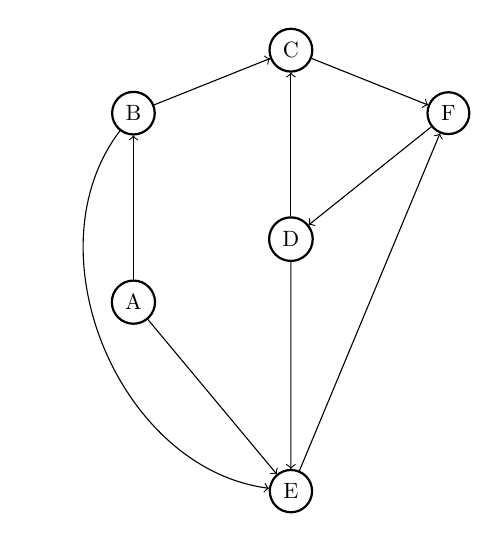
\begin{tikzpicture}[scale=0.8, transform shape]
	\begin{scope}[every node/.style={circle,thick,draw}]
		\node[] (A) at (0,0) {A};
    \node (B) at (0,3) {B};
    \node[] (C) at (2.5,4) {C};
		\node[] (D) at (2.5,1) {D};
    \node (E) at (2.5,-3) {E};
    \node (F) at (5,3) {F} ;
\end{scope}

\begin{scope}[
              every node/.style={fill=white,circle},
							every edge/.style={draw=black}]
							\path[->] (A) edge[] (B);
							\path[->] (B) edge[] (C);
							\path[->] (D) edge (C);
							\path[->] (A) edge (E);
							\path[->] (D) edge[] (E);
							\path[->] (F) edge[] (D);
							\path[->] (C) edge[] (F);
							\path[->] (E) edge (F); 
							\path[->] (B) edge[bend right=60] (E); 
\end{scope}
\end{tikzpicture}

		\column{0.605\textwidth}
		\begin{questionblock}{Is this a DAG?}
		\pause
			Is this a DAG?
			\begin{enumerate}[A.]
				\item Yes
				\item No, but if we add one edge then it is.
				\item No, but if we remove one edge then it is.
				\item No, and we need to remove more than one edge to make it one.
				\item I don't know.
			\end{enumerate}
		\end{questionblock}
		\pause
		\vspace{-10pt}
		\begin{answerblock}{All of them}
			Just remove the edge $(F,D)$.
		\end{answerblock}
	\end{columns}
\end{frame}
